\section{An exact topological boundary theorem and the six-boundary sequel}\label{sec:bipartite-subcubic}
\begin{theorem}[Bipartite subcubic boundary]\label{thm:bipartite-subcubic}
For every finite simple connected bipartite graph $G$ of maximum degree at
most three and order at least two,
\[
 \bd G=\{v:\dd(v)=1\}\ \cup\ \{v:v\text{ lies on a cycle}\}.
\]
Thus its harmonic boundary can be computed in linear time from a bridge
search, without computing all-pairs distances.
\end{theorem}
\begin{proof}
Suppose $u\notin\bd G$ and $\dd(u)=2$ or $3$. In a bipartite graph,
for any target $z$, each neighbor of $u$ is at distance exactly
$d(u,z)-1$ or $d(u,z)+1$ from $z$. If $z\ne u$, a shortest path provides
at least one closer neighbor. Two closer neighbors would give a positive
score when $\dd(u)\le3$. Hence there is exactly one closer neighbor.

Partition $V(G)\setminus\{u\}$ according to that unique first neighbor.
There cannot be an edge between two different parts. Indeed, its endpoints
have root distances differing by one, by bipartiteness. A shortest path to
the nearer endpoint followed by that edge would give the farther endpoint
another first neighbor. Therefore different neighbors of $u$ lie in
different components of $G-u$. In particular, $u$ lies on no cycle.

Conversely, if $u$ lies on no cycle, every incident edge is a bridge.
For each target other than $u$, exactly one neighbor is closer and all
other neighbors are farther. Thus $\stab(u)=2-\dd(u)$, and such a vertex
is boundary exactly when it is a leaf. Leaves themselves have stability one.
\end{proof}
Both hypotheses have sharp local counterexamples: the nonbipartite theta
graph with path lengths $1,4,4$ has two interior degree-three vertices on
cycles, while the center of the bipartite $3\times3$ grid is an interior
degree-four vertex on cycles.

\begin{theorem}[Exact reduced-order identity]\label{thm:bipartite-kernel-bound}
Let $K$ be obtained from a graph in Theorem~\ref{thm:bipartite-subcubic} by
suppressing degree-two vertices lying on no cycle. Let $B_1,\ldots,B_c$ be
its nonbridge blocks, and let $a$ be the total number of bridge incidences
at their vertices. With $b=|\bd K|$,
\[
 |V(K)|=2b-2-\sum_{j=1}^c\bigl(|V(B_j)|-2\bigr)-a\le2b-2.
\]
Equality holds exactly when $K$ is a tree all of whose nonleaves have
degree three. The bound is attained for every $b\ge2$.
\end{theorem}
\begin{proof}
Two distinct nonbridge blocks cannot share a vertex: that vertex would
have degree at least four. Their vertices are therefore disjoint. Put
$S=\sum_j|V(B_j)|$, let $\ell$ count leaves, and let $t$ count the remaining
vertices of $K$, all of degree three. The preceding theorem gives
$b=S+\ell$. Contract each nonbridge block to one node. The resulting tree
has $\ell$ degree-one vertices, $t$ degree-three vertices, and $c$ block
nodes whose total degrees are $a$. The tree degree identity gives
$\ell=t+2+a-2c$. Substituting in $|V(K)|=S+\ell+t$ proves the formula.
Every nonbridge block has at least four vertices, so any such block makes
the inequality strict. The stated trees give equality.
\end{proof}


\begin{corollary}[Constructive classification at every boundary size]
Fix $b\ge2$. Choose vertex-disjoint two-connected bipartite subcubic blocks
with total order $S\le b$. Join them in a tree whose other nodes are
$b-S$ leaves and degree-three branch vertices. At each block, attach the
incident bridges injectively to distinct degree-two vertices of the block.
Retain precisely the choices making a connected graph of order at least
two. Subdivide any bridges arbitrarily. These constructions give exactly
all connected bipartite subcubic graphs with boundary size $b$.
There are finitely many reduced kernels, all of order at most $2b-2$,
and at most $\lfloor b/4\rfloor$ nonbridge blocks.
\end{corollary}
The necessity follows from the unique block decomposition and
Theorem~\ref{thm:bipartite-subcubic}; sufficiency follows from the same
boundary formula. This supplies an all-order classification for every
boundary size within this infinite class.

\begin{theorem}[Complete six-boundary bipartite subcubic classification]
Every connected bipartite subcubic graph with six harmonic boundary vertices
is obtained by arbitrary subdivisions of bridges of exactly one of the ten
kernels in the following table. Conversely every listed kernel and every
such subdivision has boundary six.
\begin{center}
\begin{tabular}{@{}p{99mm}rr@{}}\toprule
Kernel description&Number&Order\\\midrule
Trivalent tree with six leaves; the four internal vertices induce
$P_4$ or $K_{1,3}$&2&10\\
$C_4$ with one leaf at each of two adjacent or opposite vertices&2&6\\
$C_4$ joined by one bridge to a new degree-three vertex with two leaf neighbors&1&7\\
$K_{2,3}$ with one leaf attached at a degree-two vertex&1&6\\
$K_{3,3}$ with a matching of size $0,1,2,$ or $3$ deleted&4&6\\\bottomrule
\end{tabular}
\end{center}
\end{theorem}
\begin{proof}
All vertices in nonbridge blocks count toward the six boundary vertices.
Since each such block has order at least four and blocks are disjoint,
there is at most one. If none exists, the reduced graph is one of the two
six-leaf trivalent trees. If a block has order four, it is $C_4$ and exactly
two leaves remain. The tree identity gives either two direct leaf
attachments, adjacent or opposite, or a single attached two-leaf branch.
If the block has order five, it is $K_{2,3}$ and the remaining leaf must
attach at one of its symmetric degree-two vertices. If it has order six,
there are no outside vertices. Its bipartition must have sizes three and
three, and minimum degree two means its missing edges form a matching in
$K_{3,3}$. This gives the four final entries. Bridge subdivision preserves
both the stated topology and boundary.
\end{proof}


\begin{figure}[p]
\centering
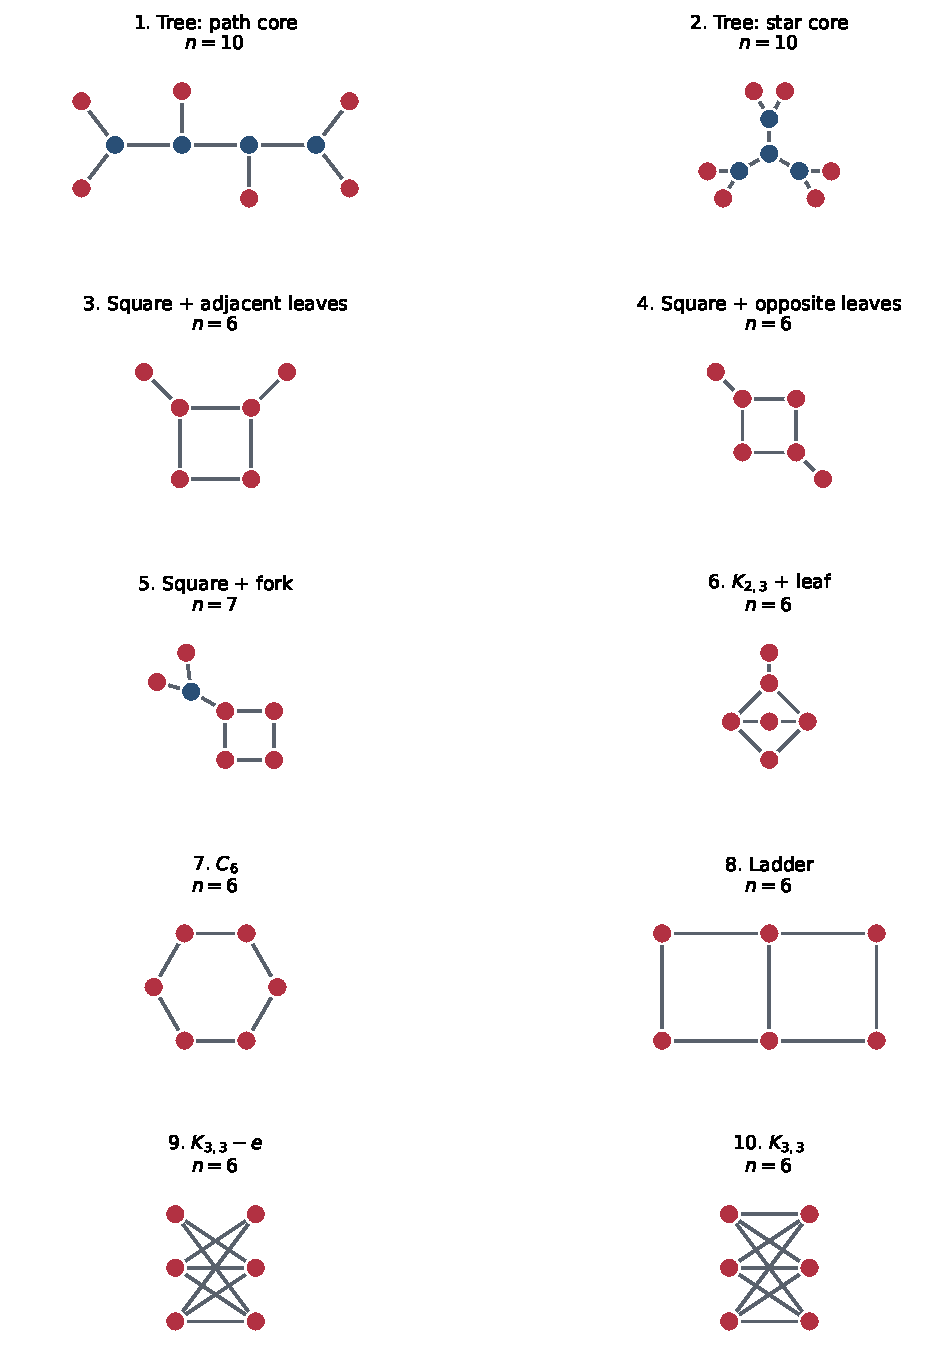
\includegraphics[width=\textwidth,height=.88\textheight,keepaspectratio]{figures/bipartite_six_kernels.pdf}
\caption{The ten bipartite subcubic six-boundary kernels. Boundary vertices
are red and interior vertices blue. Only bridges may be subdivided in this
construction; all such subdivisions are allowed. Unmarked edge crossings
are not vertices.}
\label{fig:bipartite-six-kernels}
\end{figure}

\subsection{Removing bipartiteness at boundary six}
The following section proves an all-orders reduction for nonbipartite
subcubic graphs as well, and then classifies the entire connected subcubic
six-boundary class. The bipartite theorem above remains stronger in another
direction: it applies to every boundary size and has a full graph-level
Lean proof.

For comparison, unrestricted two-connected searches at orders eight, nine,
and ten find respectively twelve, two, and one six-boundary graphs. The
last layer contains 9,743,542 graphs. This unrestricted census is only
finite evidence: the higher-degree six-boundary core problem remains open
in this work. These searches were made in the earlier session and are
not part of the package.
